\section{Results}

In this section we show how long it takes to resolve a fault over the network and we compare \projname{} to \verb,malloc, in several tests.

\subsection{Fault Handling}

There are two distinct types of faults that the \projname{} system resolves.  First, is a \em read \em fault which involves resolving a page fault that a node currently has no access to (e.g., the page permission is \verb,PROT_NONE,).  These faults involve a network message, and take significantly longer to resolve.  These faults resemble disk faults in traditional memory systems.  Second, is a \em write \em fault used for detecting when pages are dirtied.  This fault is handled quickly, and involves a minimal overhead.  No networking messages are required to resolve these types of faults.

\begin{table}[htb]
\centering
\begin{tabular}{|l | l | l | l |}
\hline
\bf{Fault Type} & \bf{Time} \\
\hline
\bf{Read} & 3.000 ms\\
\bf{Write} & 0.045 ms\\
\hline
\end{tabular}
\caption{Average metrics for resolving read and write faults.}
\end{table}

\subsection{Access Patterns}

To demonstrate the different natures and effects of coherency models, we included figure \ref{access-patters-strict} and figure \ref{access-patters-rc}.  Figure \ref{access-patters-strict} depicts the access patterns of a matrix multiply benchmark application using a \em strict \em coherency model.  This coherency model necessitates that each read or write to memory happen on the latest version of a page.  Figure \ref{access-patters-rc} depicts the access patterns of the same matrix multiply benchmark application using a \em LRC \em coherency model.  This coherency mode provides a mechanism for each node to maintain read-only pages, and necessitates the transfer of modified pages only.

One can see from the two figures the difference in access patterns.  Stricter coherency models require many more messages and faults.  This is evidence to why strict coherency models aren't typically used in DSM systems.  On the other hand, the more efficient weaker coherency models facilitate the transfer of modified pages only.  This has the advantage of requiring fewer messages and faults, and can be implemented in a lazy fashion.

\begin{figure*}[t]
\centering
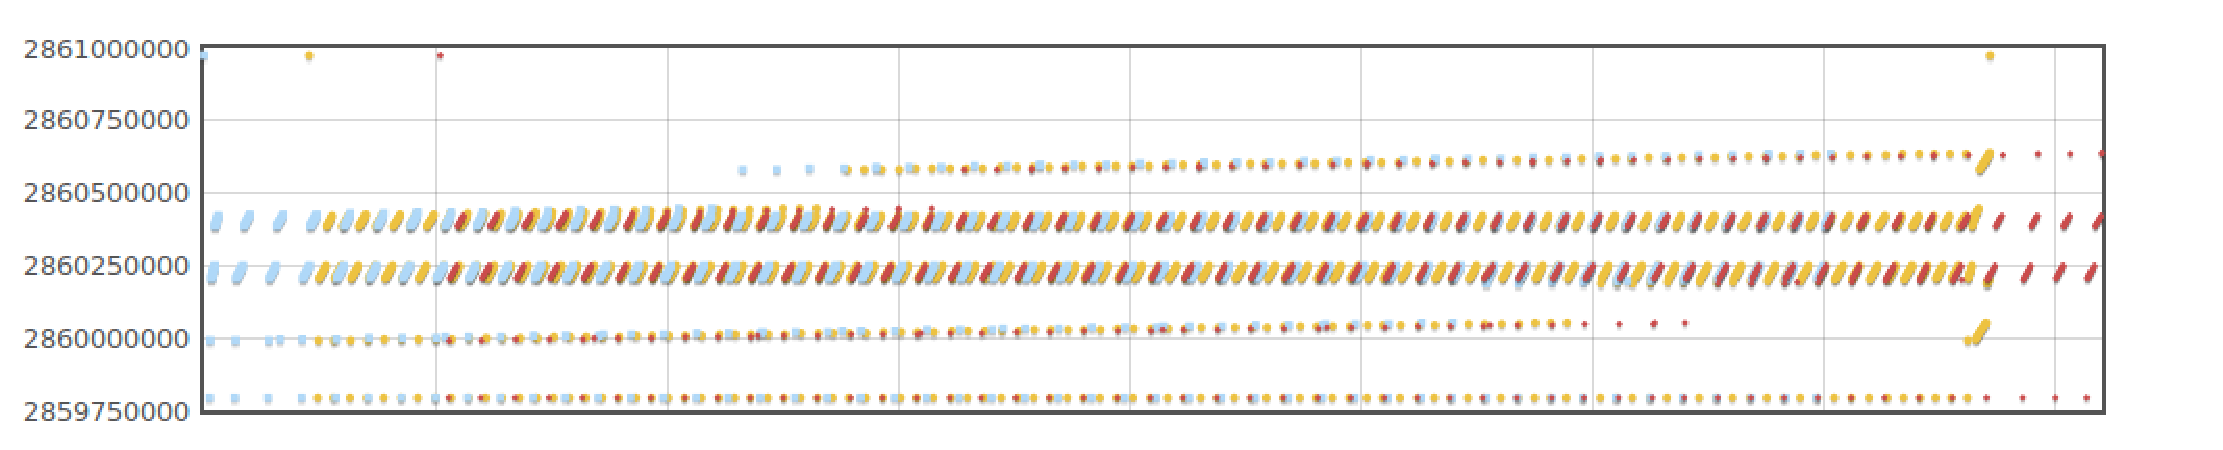
\includegraphics[scale=0.40]{images/access-patterns-strict.eps}
\caption{Access patterns exhibited by a \em strict \em coherency model during the running of a matrix multiplication benchmark application.  The vertical axis labels memory address (as an integer value).  The horizontal axis is time (values and units omitted).}
\label{access-patters-strict}
\end{figure*}

\begin{figure*}[t]
\centering
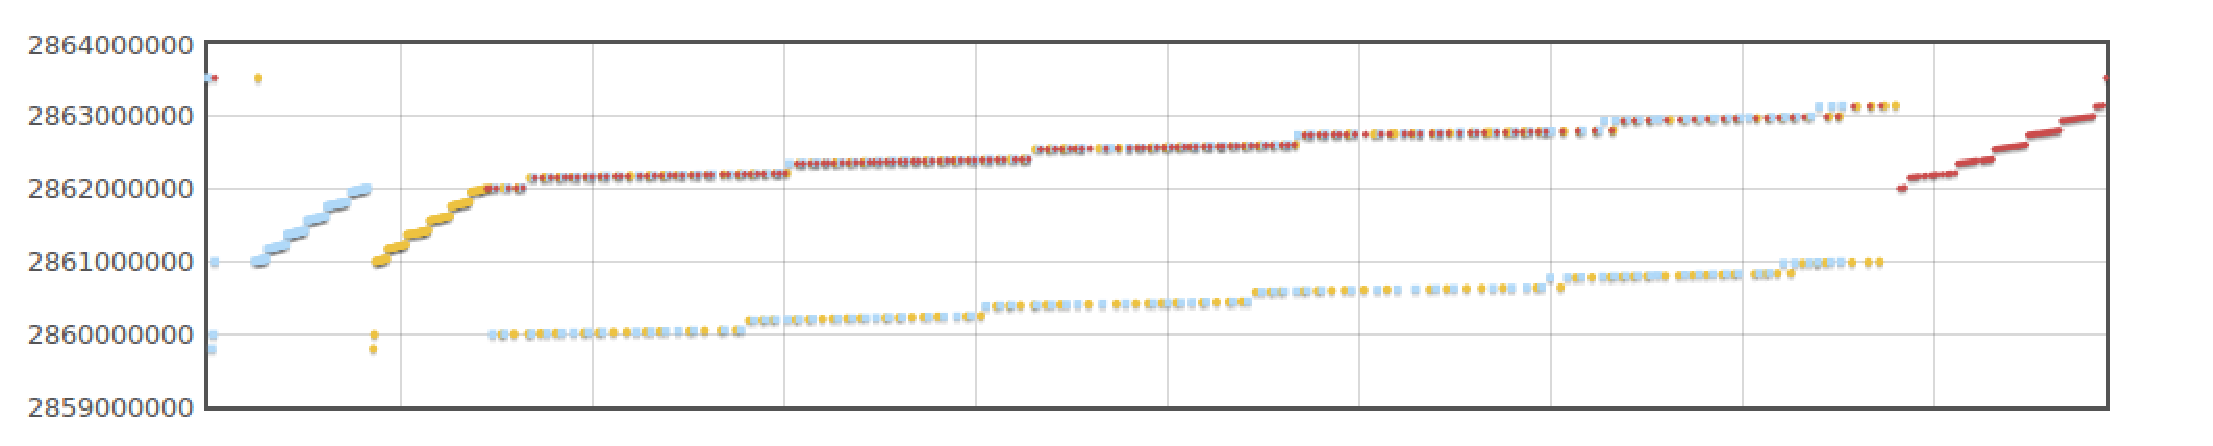
\includegraphics[scale=0.40]{images/access-patterns-rc.eps}
\caption{Access patterns exhibited by a \em LRC \em coherency model during the running of a matrix multiplication benchmark application.  The vertical axis labels memory address (as an integer value).  The horizontal axis is time (values and units omitted).}
\label{access-patters-rc}
\end{figure*}



\subsection{System Allocator VS. \projname{}}

The program used to test was a matrix multiplication program from Stanford.

\subsubsection{Fixed matrix size, varying number of threads}

In this test we kept the matrix size fixed at 200x200 and we varied the number of worker threads between 1 and 4.

\begin{figure}[!h]
\centering
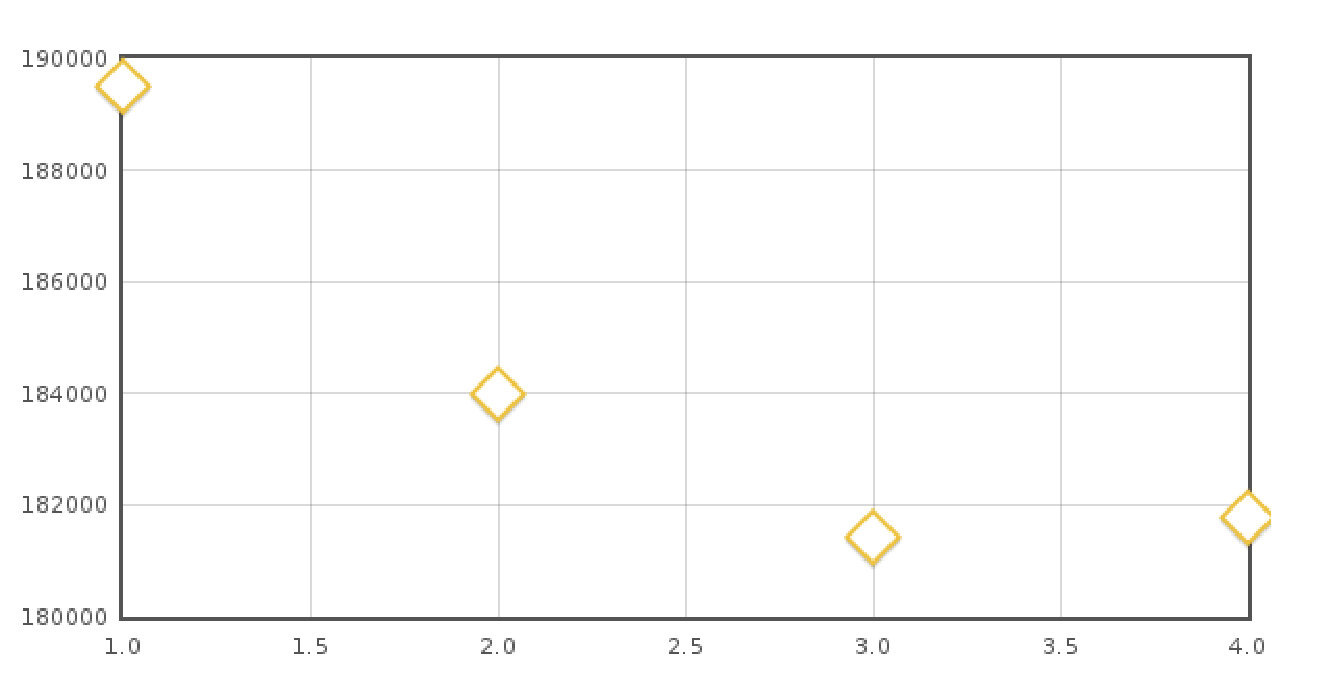
\includegraphics[scale=0.40]{images/malloc-fixed-matrix.eps}
\caption{Malloc: The x axis the number of threads used. The y axis is time to run the test in microseconds.}
\end{figure}

\begin{figure}[!h]
\centering
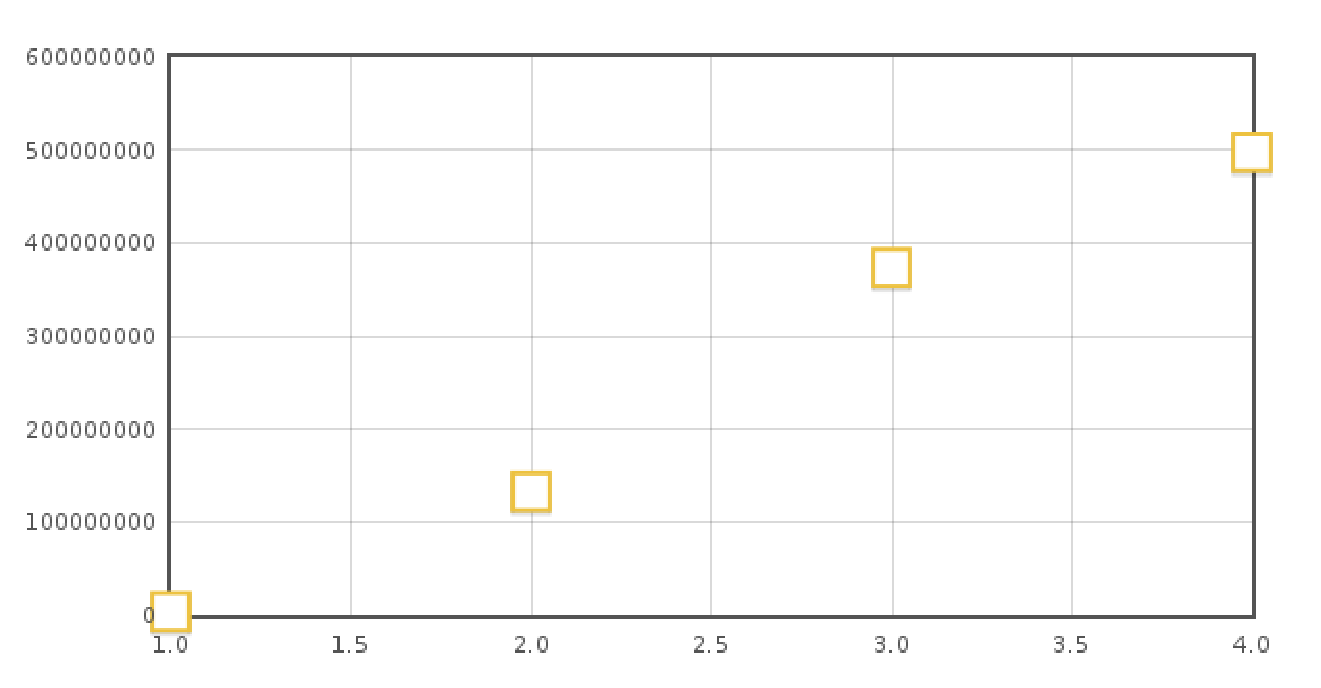
\includegraphics[scale=0.40]{images/mmult-lh-fixed-size.eps}
\caption{\projname{} with processor consistency: The x axis the number of threads used. The y axis is time to run the test in microseconds.}
\end{figure}

\begin{figure}[!h]
\centering
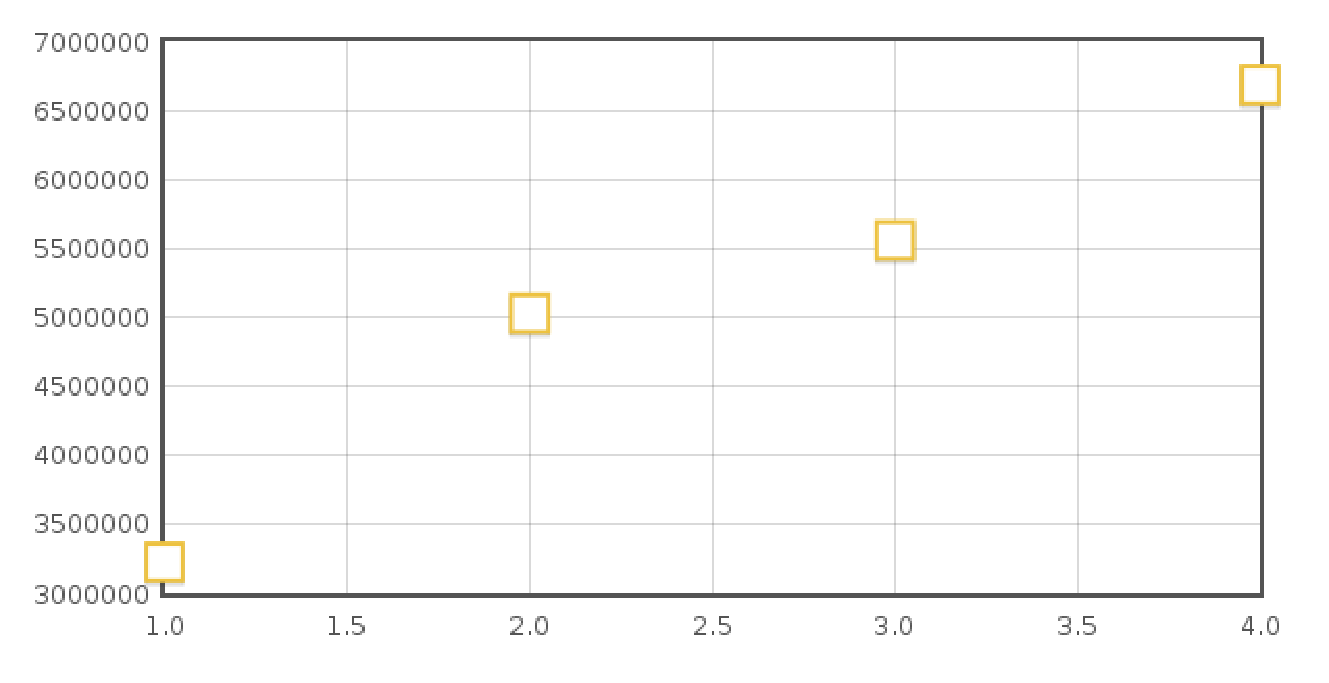
\includegraphics[scale=0.40]{images/mmlh-fixed-size.eps}
\caption{\projname{} with release consistency: The x axis is matrix size. For example, 100 refers to multiplying 2 100x100 matrices. The y axis is time to run the test in microseconds.}
\end{figure}

The system allocator, \verb,malloc(3), vastly outperforms \projname{} with processor consistency no matter how many threads are used.  This has to do with not having read-only pages.  Every time a worker needs to do work it invalidates all other workers copies of that page.  This ends up with the workers thrashing over pages.  It was expected when we began this test that \projname{} with processor consistency would yield worse results as the number of threads increased because of the trashing issues.

Using a LRC coherency model, \projname{} achieves much better performance than processor consistency.  For four worker threads, the system takes 66 seconds to execute.  Processor consistency takes around 500 seconds to execute.  Release consistency still loses to the \verb,malloc(3), version.  One reason why is because the workers end up thrashing over the write pages.

\subsubsection{Fixed thread count, varying matrix size}

In this test we kept the number of worker threads fixed at 4 and we varied the matrix size.

\begin{figure}[!h]
\centering
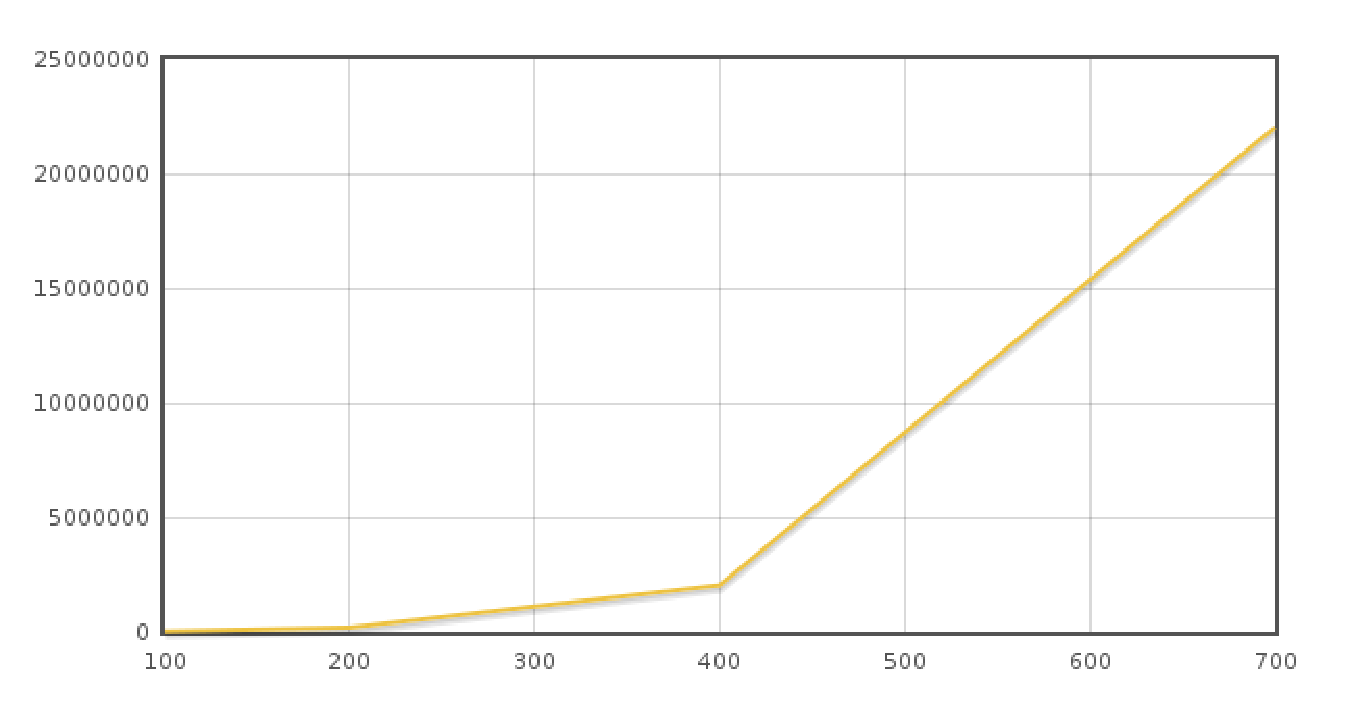
\includegraphics[scale=0.40]{images/malloc-fixed-thread.eps}
\caption{Malloc: The x axis is matrix size. For example, 100 refers to multiplying 2 100x100 matrices. The y axis is time to run the test in microseconds.}
\end{figure}

\begin{figure}[!h]
\centering
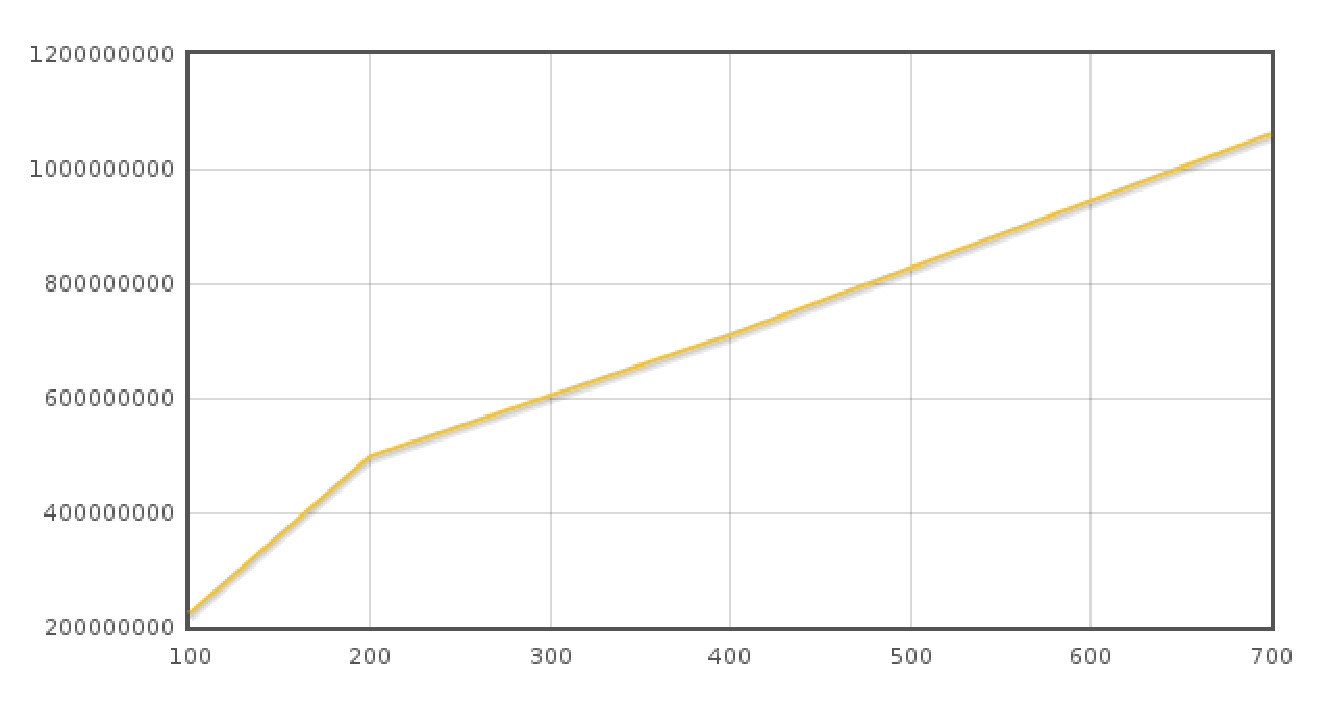
\includegraphics[scale=0.40]{images/mmult-lh-fixed-thread.eps}
\caption{\projname{} with processor consistency: The x axis is matrix size. For example, 100 refers to multiplying 2 100x100 matrices. The y axis is time to run the test in microseconds.}
\end{figure}

\begin{figure}[!h]
\centering
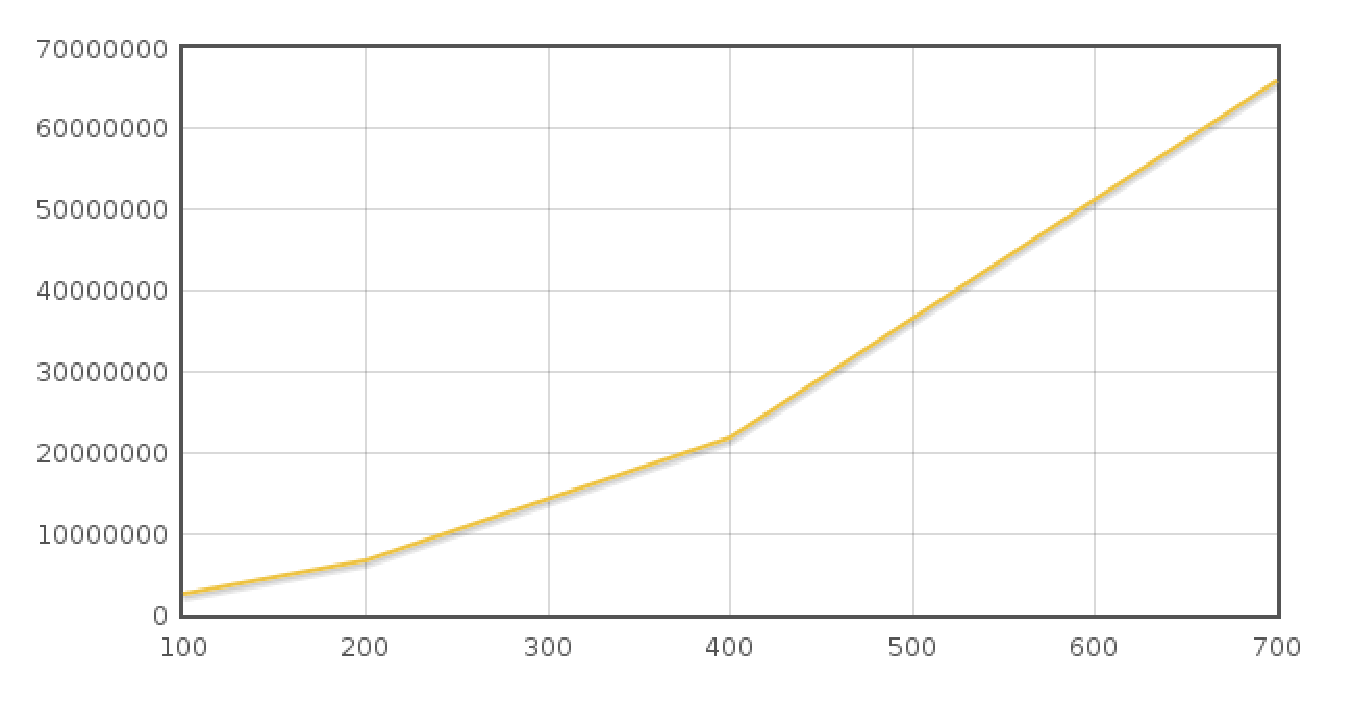
\includegraphics[scale=0.40]{images/mmlh-fixed-threads.eps}
\caption{\projname{} with release consistency: The x axis is matrix size. For example, 100 refers to multiplying 2 100x100 matrices. The y axis is time to run the test in microseconds.}
\end{figure}

Again, like in the previous test \verb,malloc, vastly outperforms \projname{} with processor consistency at any matrix size. \projname{} with processor consistency gets hit hard by not having read only pages. It ends up transferring the 2 matrices being multiplied a ton thereby having a horrific runtime.

With release consistency, \projname{} achieves much better performance than processor consistency. Again, release consistency still loses to the \verb,malloc, version because the workers end up thrashing over the write pages. It is still impressive that the release consistency version multiplying a 700x700 matrix finishes in around 66 seconds. The processor consistency version of the project was destroyed by that test and ended up taking over 1000 seconds.
